\begin{frame}{Пример — траектория дрона, 1}
	\begin{flushleft}
		
		Рассмотрим следующую задачу: спланировать траекторию для квадрокоптера, согласованную с динамикой, как квадратичную программу.
		
		\bigskip
		
		Это можно решить, используя упрощенную динамическую модель дрона, основанную на \emph{дифференциальной плоской системе}. Основная идея заключается в том, чтобы спланировать положение, скорость, ускорение и рывок центра масс (ЦМ) дрона, а затем восстановить ориентацию и угловую скорость из этой информации:
		
		\begin{itemize}
			\item Зная ускорение, можно вычислить тягу.
			\item Зная тягу, можно вычислить ориентацию (с точностью до рыскания).
			\item Зная рывок, можно вычислить угловую скорость.
		\end{itemize}
		
	\end{flushleft}
\end{frame}



\begin{frame}{Пример — траектория дрона, 2}
	\begin{flushleft}
		
		Пусть $\bo{B} = [\bo{b}_1 \ \bo{b}_2 \ \bo{b}_3]$ — матрица поворота, описывающая ориентацию квадрокоптера в мировой системе координат.
		
		\begin{figure}
			\centering
			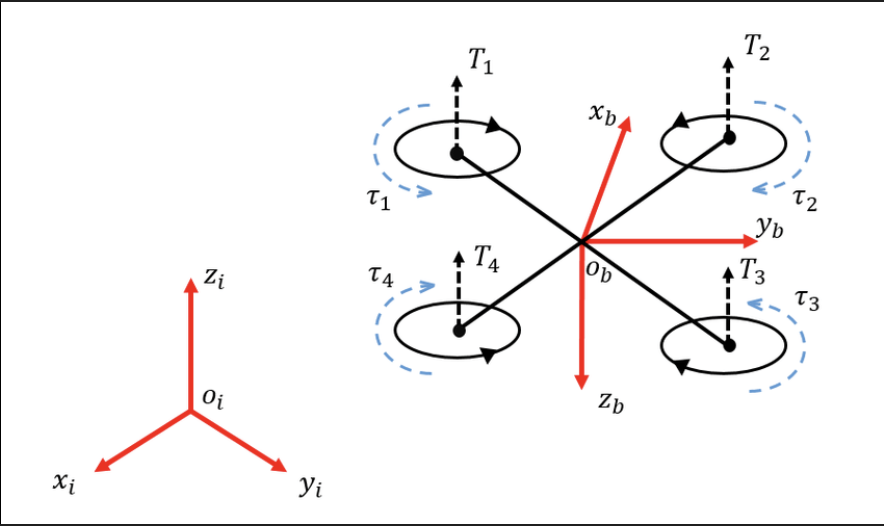
\includegraphics[width=0.7\linewidth]{drone}
			%\caption{Система координат квадрокоптера}
			\label{fig:drone}
		\end{figure}
		
		Используем следующее соглашение: $\bo{b}_1$ и $\bo{b}_2$ лежат в касательной плоскости дрона, а $\bo{b}_3$ лежит в нормальном направлении к этой плоскости; эти векторы выбраны так, чтобы они образовывали правый базис, а тяга $\bo{f}_t = -f \bo{b}_3$ (вектор $\bo{b}_3$ "направлен вниз" в связанной системе координат).
		
	\end{flushleft}
\end{frame}



\begin{frame}{Пример — траектория дрона, 3}
	\begin{flushleft}
		
		Известно, что сила тяжести в мировой системе координат выражается как $\bo{f}_g = mg \bo{e}_3$, где $\bo{e}_3 = [0 \ 0 \ 1 ]\T$ и $g \approx 9.81$.
		
		\bigskip
		
		Ускорение центра масс можно вычислить как:
		%
		\begin{align}
			m \bo{a} = \bo{f}_g + \bo{f}_t 
			\\
			m \bo{a} = mg \bo{e}_3 - f \bo{b}_3 
		\end{align}
		%
		Используя это, можно вычислить $\bo{b}_3$:
		%
		\begin{align}
			\bo{b}_3 = \frac{\bo{f}_t}{||\bo{f}_t||} =  \frac{g \bo{e}_3 - \bo{a}}{||g \bo{e}_3 - \bo{a}||}
		\end{align}
		%
		
		
		
	\end{flushleft}
\end{frame}


\begin{frame}{Пример — траектория дрона, 4}
	\begin{flushleft}
		
		Таким образом, нашими переменными являются положение $\bo{p}$, скорость $\bo{v} = \dot{\bo{p}}$, ускорение $\bo{a} = \ddot{\bo{p}}$ и рывок $\bo{j} = \dddot{\bo{p}}$. 

\bigskip

В нашей оптимизации мы можем стремиться минимизировать толчок (snap) — четвертую производную положения, производную рывка. Функция стоимости тогда примет вид:

\begin{equation}
	\boxed{
		J = \sum_{i = 1}^{N-1} ( \bo{j}_{i+1} - \bo{j}_i)\T ( \bo{j}_{i+1} - \bo{j}_i) }
\end{equation}


\end{flushleft}
\end{frame}

\begin{frame}{Пример — траектория дрона, 5}
	\begin{flushleft}
		
		Мы можем добавлять ограничения; например, можно задать определенный крен-тангаж на временном шаге $k$. Для этого опишем желаемую пару крена и тангажа через желаемое направление нормали $\bo{b}_3^\text{des}$ (желаемую ориентацию вертикальной оси квадрокоптера). 
		
		\bigskip
		
		Тогда ограничение можно записать как «векторное произведение между $\bo{b}_3$ и $\bo{b}_3^\text{des}$ должно быть равно нулю»:
		
		\begin{align}
			\bo{b}_3^\text{des} \times \bo{b}_3 = 0
			\\
			\bo{b}_3^\text{des} \times   \frac{g \bo{e}_3 - \bo{a}}{||g \bo{e}_3 - \bo{a}||} = 0
			\\
			\boxed{
				\bo{b}_3^\text{des} \times (g \bo{e}_3 - \bo{a}) = 0
			}
		\end{align} 
		
		
	\end{flushleft}
\end{frame}



\begin{frame}{Пример — траектория дрона, 6}
	\begin{flushleft}
		
		Добавляя ограничения на начальное и конечное положения, задача планирования траектории становится задачей КП:
		
		\begin{equation}
			\begin{aligned}
				& \underset{\bo{p},\bo{v},\bo{a},\bo{j}}{\text{minimize}}
				& &\sum_{i = 1}^{N-1} ( \bo{j}_{i+1} - \bo{j}_i)\T ( \bo{j}_{i+1} - \bo{j}_i), \\
				& \text{subject to}
				& & \begin{cases}
					\bo{b}_3^\text{des}(k) \times (g \bo{e}_3 - \bo{a}_k) = 0
					\\
					\bo{p}_{i+1} = \bo{p}_i + h \bo{v}_i \\
					\bo{v}_{i+1} = \bo{v}_i + h \bo{a}_i \\
					\bo{a}_{i+1} = \bo{a}_i + h \bo{j}_i 
					\\
					\bo{p}_1 = \bo{p}_1^\text{des}
					\\
					\bo{p}_N = \bo{p}_N^\text{des}
				\end{cases}
			\end{aligned}
		\end{equation}
		%
		где $h$ — шаг по времени.
		
	\end{flushleft}
\end{frame}



\begin{frame}{Пример — траектория дрона, 7 (дополнительно)}
	\begin{flushleft}
		
		
		Чтобы вычислить ориентацию $\bo{B} = [\bo{b}_1 \ \bo{b}_2 \ \bo{b}_3]$ по $\bo{a}$, используем следующие шаги:
		
		\begin{enumerate}
			
			\item Вычисляем $\bo{b}_3 =  \frac{g \bo{e}_3 - \bo{a}}{||g \bo{e}_3 - \bo{a}||}$.
			
			\item Выбираем опорное значение рыскания $\psi$ и $\bo{b}_\text{yaw} = \begin{bmatrix}
				\cos (\psi) & \sin(\psi) & 0
			\end{bmatrix}\T$.
			
			\item Вычисляем $\bo{b}_2$ через ортогональность и нормировку: $\bo{b}_2 = \frac{\bo{b}_3 \times \bo{b}_\text{yaw}}{||\bo{b}_3 \times \bo{b}_\text{yaw}||}$
			
			\item Завершаем базис: $\bo{b}_1 =  \bo{b}_2 \times \bo{b}_3$.
		\end{enumerate}
		
	\end{flushleft}
\end{frame}



\begin{frame}{Пример — траектория дрона, 8 (дополнительно)}
	\begin{flushleft}
		
		
		Чтобы вычислить угловую скорость (в связанной системе координат) $\omega = \begin{bmatrix}
			\omega_x & \omega_y & \omega_z
		\end{bmatrix}\T$ по $\bo{j}$, используем следующие шаги:
		
		\begin{enumerate}
			
			\item Вычисляем $\dot{ \bo{b}}_3 =  -\frac{1}{||\bo{f}_t||}(\bo{I} - \bo{b}_3 \bo{b}_3\T) \bo{j}$. \textcolor{mygray}{Используем тот факт, что $\bo{b}_3 = -\frac{\bo{f}_t}{||\bo{f}_t||}$ — единичный вектор.}
			
			\item Вычисляем $\omega_x = - \bo{b}_2\T \dot{ \bo{b}}_3$ и $\omega_y = \bo{b}_1\T \dot{ \bo{b}}_3$.
			
			\item Выбираем $\omega_z = \dot \psi$.
		\end{enumerate}
		
		\bigskip
		
		\textcolor{mygray2}{
			Заметим, что $\omega = \omega_x \bo{b}_1 + \omega_y \bo{b}_2+ \omega_z \bo{b}_3$, следовательно $\dot{ \bo{b}}_3  = \omega \times \bo{b}_3 = ( \omega_x \bo{b}_1 + \omega_y \bo{b}_2) \times \bo{b}_3$. Поскольку $ \bo{b}_1 \times  \bo{b}_3 =  -\bo{b}_2$ и $ \bo{b}_2 \times  \bo{b}_3 =  \bo{b}_1$, получаем $\dot{ \bo{b}}_3  =  -\omega_x \bo{b}_2+ \omega_y \bo{b}_1$. Проецируя, получаем формулы выше.}
		
	\end{flushleft}
\end{frame}